\cleartooddpage[\thispagestyle{empty}]


\newcommand{\Lim}[1]{\raisebox{0.5ex}{\scalebox{0.8}{$\displaystyle \lim_{#1}\;$}}}
\renewcommand{\labelitemi}{\textbullet}
\newcommand{\pip}[1]{$\pi^{+}$}
\newcommand{\pim}[1]{$\pi^{-}$}
\newcommand{\pio}[1]{$\pi^{0}$}
\newcommand{\sv}{\left < \sigma v \right >}

\chapter{Gamma Rays and Dark Matter}\label{ch_gamma}


This thesis searches for evidence of dark matter within gamma ray data, but the relationship between these two areas of physics is intricate.
In this chapter three topics relevant to this relationship are discussed.
The first is the astrophysical mechanisms that can produce TeV-energy gamma rays, a background for detecting dark matter gamma rays.
The second is how dark matter around the Galactic Center can produce gamma rays.
The third topic is how gamma rays induce air showers in the Earth's atmosphere.

\section{Production of TeV Gamma Rays}

  There are several mechanisms that can produce photons with TeV energies.
  A gamma ray can start as a low-energy photon, then gain significant energy from electroweak interactions with electrons, referred to as a leptonic production.
  Alternately, a gamma ray can be created from a high-energy proton colliding with another proton, which produces neutral pions ($\pi^0$'s) that decay into gamma rays.
  This is referred to as hadronic production.
  However, leptonic and hadronic production are separate from how gamma rays are produced by dark matter.
  Instead, two WIMP dark matter particles may annihilate (directly or indirectly) into gamma rays, and this is discussed in Section~\ref{dm_spectral}.

  In leptonic production, electrons and low-energy photons collide, transferring energy to the photon.
  This interaction is called inverse Compton scattering (or occasionally upscattering)~\cite{compton_effect}, and its Feynman diagram is shown in Figure~\ref{fig:inv_compt_feyn}.
  
  \begin{figure}[!ht]
    \centering
    \includegraphics[width=0.45\textwidth]{images/feynman_particles/inversecompton.pdf}
    \caption[Inverse Compton Scattering Feynman Diagram]{
      Feynman diagram of inverse Compton scattering, where an electron upscatters a low-energy photon (red) to produce a higher-energy (blue) photon.
    }
    \label{fig:inv_compt_feyn}
  \end{figure}
  \FloatBarrier
  
  In inverse Compton scattering~\cite{inv_compt1,inv_compt2}, a field of photons with an electron present will gain energy according to 
  
  % https://eud.gsfc.nasa.gov/Volker.Beckmann/school/download/Longair_Radiation3.pdf equation 11
  \begin{equation}\label{eqn:inv_compt_en_gain_rate}
    \frac{dE}{dt} = \frac{4}{3} \: \sigma_{t} \: U \: c \: \gamma^2 \: \frac{ v^2 }{ c^2 } \;\; ,
  \end{equation}
  where
  
  \begin{itemize}
    \item $\sigma_{t}$ is the Thomson cross section, $\frac{8\pi}{3} \left ( \frac{\alpha \hbar c}{m c^2} \right )$,
    % Thomson cross section is from wikipedia.org/wiki/Thomson_scattering
    \item $c$ is the speed of light in vacuum,
    \item $\gamma$ is the Lorentz factor,
    \item $U$ is the energy density of the photon field in the rest frame of the electron (e.g. $Uc=N\hbar \omega c$), and 
    \item $v$ is the velocity of the electron in the laboratory frame.
  \end{itemize}
  The average energy $E_{up}$ of photons upscattered this way can be calculated via
  
  % https://eud.gsfc.nasa.gov/Volker.Beckmann/school/download/Longair_Radiation3.pdf equation 15
  \begin{equation}\label{eqn:inv_compt_avg_up_en}
    E_{up} = \frac{4}{3} \: \gamma^2 \: E_{0} \,,
  \end{equation}
  where the parameter $E_{0}$ is the energy of the original photon.
  
  % me = 5e5 eV (mass of electron)
  
  % formula for calculating gamma (lorentz factor) from relativistic kinetic energy
  % Ek = mc^2 / sqrt(1-v^2/c^2) - mc^2
  % Ek + mc^2 = mc^2 / sqrt(1-v^2/c^2)
  % ( Ek + mc^2 ) / mc^2 = 1 / sqrt(1-(v^2/c^2)) = g
  
  % lorentz factor for various kinetic energy electrons
  % Ek = 5e5  eV, 500 KeV, g =   2
  % Ek = 1e6  eV,   1 MeV, g =   3
  % Ek = 1e7  eV,  10 MeV, g =  21
  % Ek = 1e8  eV, 100 MeV, g = 201
  % Ek = 1e9  eV,   1 GeV, g = 2e3
  % Ek = 1e10 eV,  10 GeV, g = 2e4
  % Ek = 5e11 eV, 500 GeV, g = 1e6
  
  % calculating the energy in eV of a green photon
  % lg = 550e-9 m  = 5.5e-7 m
  % c = l*w
  % wg = c / lg
  % wg = 2.99e8 m/s / 5.5e-7 m = 5.4e14 1/s
  % E  = hbar w
  % hbar = 1.05e-34 m^2 kg / s (reduced planck constant)
  % 1 J = 6.24e18 eV
  % Eg = hbar wg
  % Eg = 1.05e-34 m^2 kg / s    * 5.4e14 1/s * 6.24e18 eV/J
  % Eg = 1.05 * 5.4 * 6.24 e-34 e14 e18 eV
  % Eg = 35.3e-2 eV
  % Eg = 0.35 eV (energy of a green photon)
  
  % 500 GeV electron upscatters a 0.35 eV photon (green) into a ? eV photon?
  % gamma = (Ek + Ee) / Ee
  % gamma = ( 5e11 eV + 5e5 eV ) / 5e5 eV
  % gamma = 1e6
  % Eup = (4/3) * gamma^2 * Eg
  % Eup = (4/3) * 1e12 * 0.35 eV
  % Eup = 4.67e11 eV = 467 GeV
  
  Astrophysical electrons have been detected at Earth at energies of \SI{500}{\GeV{}}~\cite{500GeVElectrons,fermi_electron}, and potentially as high as \SI{20}{\TeV{}}~\cite{hess2017_electronspectrum}.
  At energies of \SI{500}{\GeV{}}, the Lorentz factor is $\gamma = 10^6$.
  With this Lorentz factor, upscattered photons can increase their energy by up to\footnote{This is the maximum average energy gain when the upscattered photon is emitted back along its original trajectory.} $\gamma^{2} = 10^{12}$.
  For example, a green photon ($\lambda_{\textrm{green}}=550\,\textrm{nm}$, $E_{\textrm{green}}=0.3\,\textrm{eV}$) could be upscattered to as high as \SI{467}{\GeV{}}, becoming a gamma ray detectable by VERITAS.
  
  In order to efficiently produce gamma rays via this method, a population of high-energy electrons is needed.
  One environment that produces these electrons is pulsar wind nebulae.
  Because pulsars spin rapidly, they produce strong magnetic fields.
  For example, the pulsar at the heart of the Crab nebula has a surface magnetic field strength of \SI{e12}{G}~\cite{pwn_evolution}, much larger than Earth's $\sim$\SI{0.5}{G}~\cite{earth_geomag}.
  These strong magnetic fields provide an environment for producing and accelerating charged particles.
  In these strong magnetic fields, ambient photons can convert into $e^{+}e^{-}$~\cite{pwn_pairprod2,pwn_pairprod3}.
  The probability $\Upsilon$ (0-1) of a photon pair-converting in a magnetic field is calculated by via 
  
  \begin{equation}\label{eqn:pwn_pairprod}
    \Upsilon = \frac{E}{mc^2} \frac{H}{c} \frac{e \hbar}{m^2c^2} \,,
  \end{equation}
  where $E$ is the photon energy, $H$ is the ambient magnetic field strength, $e$ is the electron charge, and $m$ is the mass of the electron~\cite{pwn_pairprod3}.
  The factor $\frac{e \hbar}{m^2c^2}$ acts as a threshold magnetic field strength, above which the conversion rate becomes significant.
  For electrons the threshold is $\frac{1}{4.4\times10^{13}\,\textrm{Gauss}}$, similar in scale to the pulsar's surface magnetic field strength.
  %
  % paper : https://journals.aps.org/rmp/pdf/10.1103/RevModPhys.38.626
  % High-Energy Electromagnetic Conversion Processes in Intesnse Magnetic Fields, T. Erber, 1966
  %    NOTICE: This paper has a mistake in equations 1.1 and 1.1a (a 'c' in 1.1a should be moved to 1.1, thats all)
  %
  % e = 1.602e-19 C
  % hbar = 1.05e-34 J*s
  % m_electron = 9.11e-31 kg
  % c = 2.98e8 m/s
  % 1 Gauss = 1e-4 kg/ A*s^2 = 1e-4 kg C^-1 s^-1
  % 
  % factor = e hbar / m^2 c^2
  %        = 1.602e-19 C * 1.05e-34 J*s / (9.11e-31 kg)^2 (2.98e8 m/s)^2
  %        = 4.4e13 G
  
  Charged particles can also be accelerated by a pulsar's magnetic fields, in a process called magnetic reconnection, shown in Figure~\ref{fig:magcon}.
  In this mechanism, two oppositely oriented magnetic fields move towards each other (Figure~\ref{fig:magcon}.a), due to the field lines being frozen into the local plasma.
  As the magnetic field lines merge (Figures \ref{fig:magcon}.b and c), induced current flows produce electric fields (Figure~\ref{fig:magcon}.d) that can accelerate charged particles~\cite{magcon_crab,magcon_schopper,magcon_review,gamma_pwn1,gamma_pwn2,magconsim2011,magconsim2014,magcon_particleaccel}.
  
  \begin{figure}[!t]
    \centering
    \begin{tabular}{m{1cm}m{10cm}}
      (a) & \includegraphics[width=0.5\textwidth]{images/magnetic_reconnection/diagram_1_cr.pdf} \\
      (b) & \includegraphics[width=0.5\textwidth]{images/magnetic_reconnection/diagram_2_cr.pdf} \\
      (c) & \includegraphics[width=0.5\textwidth]{images/magnetic_reconnection/diagram_3_cr.pdf} \\
      (d) & 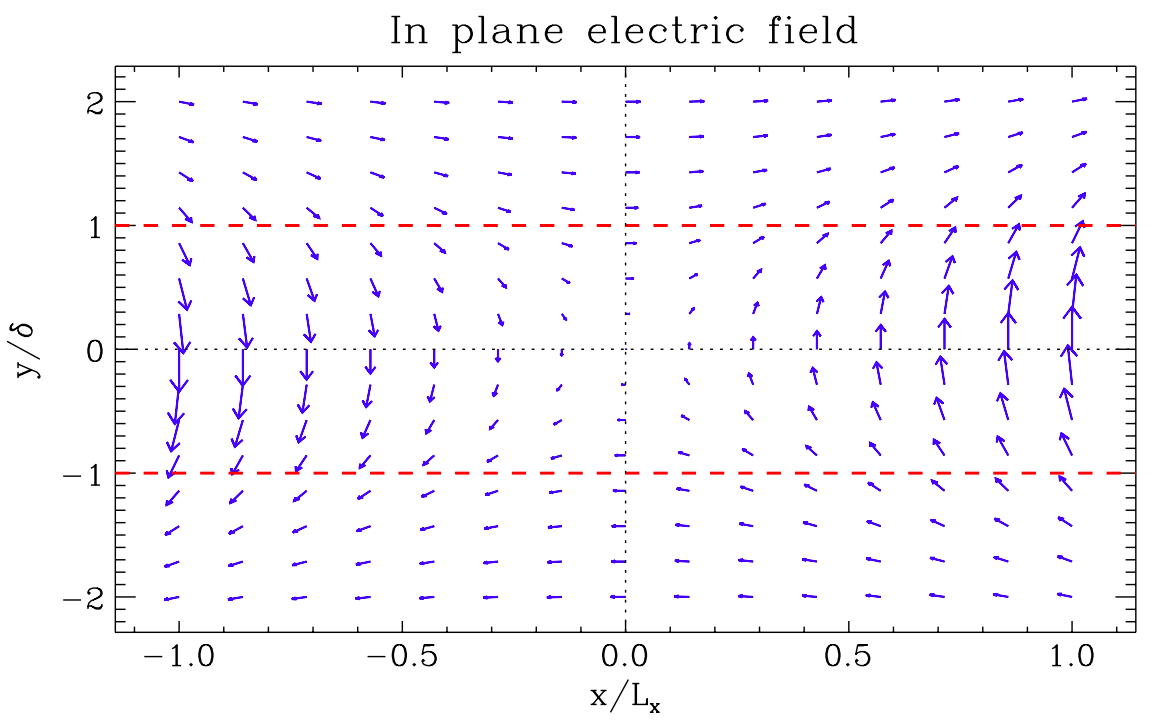
\includegraphics[width=0.5\textwidth]{images/magnetic_reconnection/magcon_efieldlines.pdf}
    \end{tabular}
    \caption[Magnetic Reconnection]{
      Reconnection of two magnetic fields.
      In (a), two oppositely-pointing magnetic fields move into each other.
      In (b), reconnection starts to occur.
      In (c), reconnection occurs, and plasma moves outwards along the $y=0$ axis.
      In (d), the resulting electric fields from the moving plasma are shown in this scenario, from Ref.~\cite{magcon_crab}.
      In these figures, $\delta$ and $\textrm{L}_{\textrm{x}}$ are the distance parameters of the reconnection area.
    }
    \label{fig:magcon}
  \end{figure}
  
  
  \FloatBarrier
  % Use figure 2 in http://iopscience.iop.org/article/10.1088/0004-637X/746/2/148/pdf
  
  % Use these sources, to get an idea of the electric field strengths doing the accelerating
  % http://iopscience.iop.org/article/10.1088/0004-637X/746/2/148/pdf
  % https://aip.scitation.org/doi/pdf/10.1063/1.873696
  % https://www.annualreviews.org/doi/pdf/10.1146/annurev-astro-082708-101726
  % something is still missing, can't find complete description of E field
  
  
  
  %The electric field in Figure~\ref{fig:magcon}.d is able to accelerate charged particles, and can be calculated with Equation~\ref{eqn:magcon_efield},
  %\begin{equation}\label{eqn:magcon_efield}
  %  \hat{E} = -\hat{V} \times \frac{B_{z}}{c} \;\; .
  %\end{equation}
  %In Equation~\ref{eqn:magcon_efield}, 
  %\begin{equation}
  %  \hat{V} = \left ( c \frac{x}{L_x} \cosh^{-2} \left ( \frac{y}{\delta} \right ),-c\beta \tanh \left ( \frac{y}{\delta} \right ), 0 \right )
  %\end{equation}
  %From \cite{magcon_crab}, equations (2) and (3).
  % 
  %\begin{equation}
  %  \hat{B} = \left ( B_0 \tanh \left ( \frac{y}{\delta} \right ), \beta B_0 \frac{x}{L_x}, 0 \right )
  %\end{equation}
  %From \cite{magcon_crab}, equations (1) and (4).
  % 
  %But this results in:
  %\begin{equation}
  %  \hat{E} = \left (  0, 0, B_0 \frac{x^2}{L_x} \beta \sech \frac{y}{\delta}^2 - B_0 \beta \tanh \frac{y}{\delta}^2 \right )
  %\end{equation}
  %Which doesn't match the plot in Figure~\ref{fig:magcon}.d .

  Another mechanism that produces high-energy charged particles is Fermi acceleration~\cite{fermi1949,highenergyelectron_snr}.
  In general, this acceleration imparts energy to charged particles when they are reflected by an oncoming magnetic field.
  
  One environment where this can happen often is in the shockfront of a supernova, where the process is called diffusive shock acceleration~\cite{dsa1,dsa2,dsa3,dsa4,dsa5}.
  During and after a supernova's initial explosion, charged fermions are quickly heated.
  These heated particles then expand outwards, creating a moving shockfront at the boundary between the expanding particles and the surrounding Inter-Stellar Medium (ISM).
  These expanding particles bring their own magnetic fields due to Alfven's theorem~\cite{alfven1,alfven2}, which then reflect other charged particles.
  % MHD for astrophysicists: https://wwwmpa.mpa-garching.mpg.de/~henk/mhd12.pdf
  %    see equation 1.27 and surrounding paragraphs
  % from wikipedia https://en.wikipedia.org/wiki/Alfv%C3%A9n%27s_theorem
  %    "For the perpendicular motions of the fluid, the field lines will push the fluid or otherwise they will be dragged with the fluid."
  % from https://warwick.ac.uk/fac/sci/physics/research/cfsa/people/valery/teaching/khu_mhd/KHU_mhd_handout.pdf , pg 23
  %   "Consequently, the magnetic field lines are frozen into the plasma: plasma can move freely along field
  %     lines, but, in motion perpendicular to them, either the field lines are dragged with the plasma or the field
  %     lines push the plasma."
  %   However:
  %     "Alfv´en’s Theorem prohibits reconnection of magnetic field lines."
  As the shockfront expands, it also runs into the ambient magnetic fields in the ISM, which can also reflect charged particles.
  This shockfront is shown in Figure~\ref{fig:snr_shockfront}.

  \begin{figure}[!t]
    \centering
    \includegraphics[width=0.75\textwidth]{images/snr_shockfront/shockfront_diagram.pdf}
    \caption[Supernova Shockfront]{
      Diagram of supernova shockfront.
      Relative to some inertial observer, the supernova plasma expands at velocity $v_s$, while the ISM moves at velocity $v_m$.
    }
    \label{fig:snr_shockfront}
  \end{figure}
  
  At the shockfront, particles that cross it are reflected off the magnetic fields on the other side, gaining a small amount of energy each time.
  Over many crossings, charged particles can gain high energies, though the higher the energy of the particle, the more likely it is to escape the shockfront, since it's gyroradius increases as its energy increases.
  The amount of energy gained is governed by a parameter $\beta$, in the equation
  
  \begin{equation}\label{eqn:snr_beta}
    \beta = 1 + \frac{v_s}{c} \,.
  \end{equation}
  This $\beta$ parameter can be interpreted as the fractional energy gain per crossing, as in

  \begin{equation}\label{eqn:snr_beta_en}
    E_{i+1} = \beta E_{i} \,,
  \end{equation}
  where the $E_i$ parameter is the average energy of a charged particle after it's $i^{\textrm{th}}$ crossing.
  The energy gain $\beta$ factor influences the energy spectrum of the escaping charged particles, but so too does $P$, the probability that the charged particle remains trapped at the shockfront after each crossing.
  This probability $P$ can be calculated with
  
  \begin{equation}\label{eqn:snr_prob}
    P = 1 - \frac{v_s}{c} \,.
  \end{equation}

  With this probability $P$ and the energy gain $\beta$, the energy spectrum of particles that permanently escape the shockfront can be calculated by
  
  \begin{equation}\label{eqn:snr_spec}
    \frac{dN}{dE} \approx E^{ \frac{\log P}{\log \beta} - 1 } \,.
  \end{equation}
  With Equations~\ref{eqn:snr_beta} and \ref{eqn:snr_prob}, the spectrum from Equation~\ref{eqn:snr_spec} can be simplified with the following substitution:

  \begin{equation}\label{eqn:snr_simplify}
    \begin{split}
       \log P     & = \log \left ( 1 - \frac{v_s}{c} \right ) \approx - \frac{v_s}{c} \\
       \log \beta & = \log \left ( 1 + \frac{v_s}{c} \right ) \approx + \frac{v_s}{c} \;\; .\\
    \end{split}
  \end{equation}
  Using Equation~\ref{eqn:snr_simplify}, Equation~\ref{eqn:snr_spec} can then be simplified to
  
  \begin{equation}\label{eqn:snr_spec_final}
    \begin{split}
      \frac{dN}{dE} & \approx E^{ \frac{\log P}{\log \beta} - 1 } \\
                    & \approx E^{ \frac{ -\frac{v_s}{c} }{ +\frac{v_s}{c} } - 1 } \\
                    & \approx E^{ -1 - 1 } \\
      \frac{dN}{dE} & \approx E^{ -2 } \;\; .
    \end{split}
  \end{equation}

  In Equation~\ref{eqn:snr_spec_final}, the exponent is often referred to as the spectral index $\gamma$.
  From this diffusive shock acceleration, the spectral index of charged particles is approximately -2.
  This is quite close to the observed extragalactic cosmic ray spectral index range of -2.0 to -2.2, but additional effects (discussed in Ref.~\cite{cosmicrayspectrumorigin}) may soften this index to get to the observed galactic cosmic ray spectral index of $\approx{}-2.7$.
  The spectral index's dependence on $P$ and $\beta$ is shown in two plots in Figure~\ref{fig:snr_spectrum}.
  The top plot in Figure~\ref{fig:snr_spectrum} shows how changing $\beta$, the energy gain per shockfront crossing cycle, affects the escape probability.
  The bottom plot shows the differential spectra using the spectral indices from the top plot.
  From these two plots, it can be seen that increasing the energy gain per crossing cycle $\beta$ creates a harder spectrum of particles with more higher energy particles, since they can reach escape energies in fewer cycles.
  It can also be seen that trapping more particles at the shockfront (higher $P$) also creates a harder spectrum of escaping particles, as particles can be contained for more cycles, gaining more energy before escaping~\cite{dsa6}.

  \begin{figure}[!p]
    \centering
    \includegraphics[width=0.7\textwidth]{images/snr_shockfront/snr_spectrum.pdf}
    \caption[Supernova Diffuse Acceleration Spectral Indices]{
      The top plot shows the spectral indices produced by various combinations of $\beta$, the fractional energy gained by a particle in one crossing cycle (upstream $\rightarrow$ downstream $\rightarrow$ upstream), and $P$, the average chance a particle is unable to escape the shockfront.
      The contours for three spectral indices $\gamma$ are shown.
      For example, at the orange triangle, each crossing cycle increases a particles energy by a factor of 1.10, while it has a 90\% chance of being permanently trapped, which produces particles with a spectral index of $\gamma=-2.1$.
      The bottom plot shows the differential flux produced by power laws with the three spectral indices shown in the top plot.
    }\label{fig:snr_spectrum}
  \end{figure}
  
  \FloatBarrier
  
  % slides on supernova shockwaves
  % https://isapp2012paris.sciencesconf.org/conference/isapp2012paris/Stefano_Gabici_three.pdf
  
  % Drury, 2012, "Origin of Cosmic Rays"
  % https://doi.org/10.1016/j.astropartphys.2012.02.006
  % Diffusive shock acceleration, 
  
  % https://www.annualreviews.org/doi/pdf/10.1146/annurev.aa.22.090184.002233 , pg 435:
  %   2 shockfronts, travelling at v1 and v2= v1 * 3/4
  %   v1 = B1 * c # velocity of the collisionless shockfront (just the B fields)
  %   v2 = B2 * c # velocity of the gas particles
  %   1 crossing cycle = reflect off each shock once = E * B2 * 4/3 increase in particle energy
  %   particle tends to escape after (B1-B2)*1/4 crossing cycles


  
  Both of these processes, magnetic reconnection and diffusive shock acceleration, can accelerate protons, electrons, or any other charged particles.
  When these processes produce electrons with high energies, these electrons can then upscatter ambient photons to TeV energies.
  Additionally, electrons spiralling through magnetic fields can produce synchrotron photons at X-ray energies, meaning fewer upscatters are needed to reach TeV energies~\cite{self_compton}.

  In hadronic processes, protons can be accelerated ($p_{accel}$) by Fermi acceleration, by a supernova remnant~\cite{proton_snr_accel}, or as part of an active galactic nucleus jet~\cite{hadronic1,hadronic2}.
  % orel commented that a sentence should be added saying that protons can be accelerated in the same way as the electrons discussed earlier
  Then, upon striking an ambient proton ($p_{ambient}$), the interaction can, in some cases, produce $\pi^{+}\pi^{+}\pi^{0}$, and other particles $X$~\cite{pp_pion,pp_pion2,pp_pion3} with
  
  %\begin{equation}\nonumber
    $$ p_{accel} + p_{ambient} \rightarrow \pi^+ + \pi^+ + \pi^0 + X \,.$$
  %\end{equation}
  The $\pi^{0}$ then quickly (\SI{8.5e-17}{s}~\cite{pdg2016}) decays into two gamma rays.
  Because each pion resulting from the original $pp$ interaction tends to receive roughly $\frac{1}{3}$ of the original proton's kinetic energy, and the $\pi^0$ decays into two gamma rays, each gamma ray ends up with \nicetilde$15\%$ of the original proton's kinetic energy.
  The X ends up possessing only a small amount of energy compared to the mass of the pions.
  For example, a proton with \SI{10}{\TeV{}} of kinetic energy will eventually produce two \SI{1.5}{\TeV{}} gamma rays.
  
  While other products from the $pp$ interaction may also produce gamma rays, the $\pi^0$ decay is the dominant production channel.
  Much of the diffuse gamma-ray component of the galactic disk is due to extra-galactic high-energy protons colliding with the protons of the galactic plane~\cite{GalacticDiffuseGammaRays,extragalactic_agn}.
  
  Protons accelerated by these mechanisms form the majority of the showers detected by the VERITAS telescope, forming an irreducible background in the Galactic Center observations.
  This background is irreducible due to the fact that the Cherenkov images of proton and gamma-ray air showers have many similarities, and cannot be identified with perfect accuracy.
  
  \subsection{Dark Matter Interactions}\label{dmgammaproduction}
    
    The general dark matter particle searched for in this thesis is a WIMP.
    WIMPs may be detectable by three general search schemes, illustrated in Figure~\ref{fig:3_searches}.

    % add popular figure for the three detection type
    \begin{figure}[!h]
      \centering
      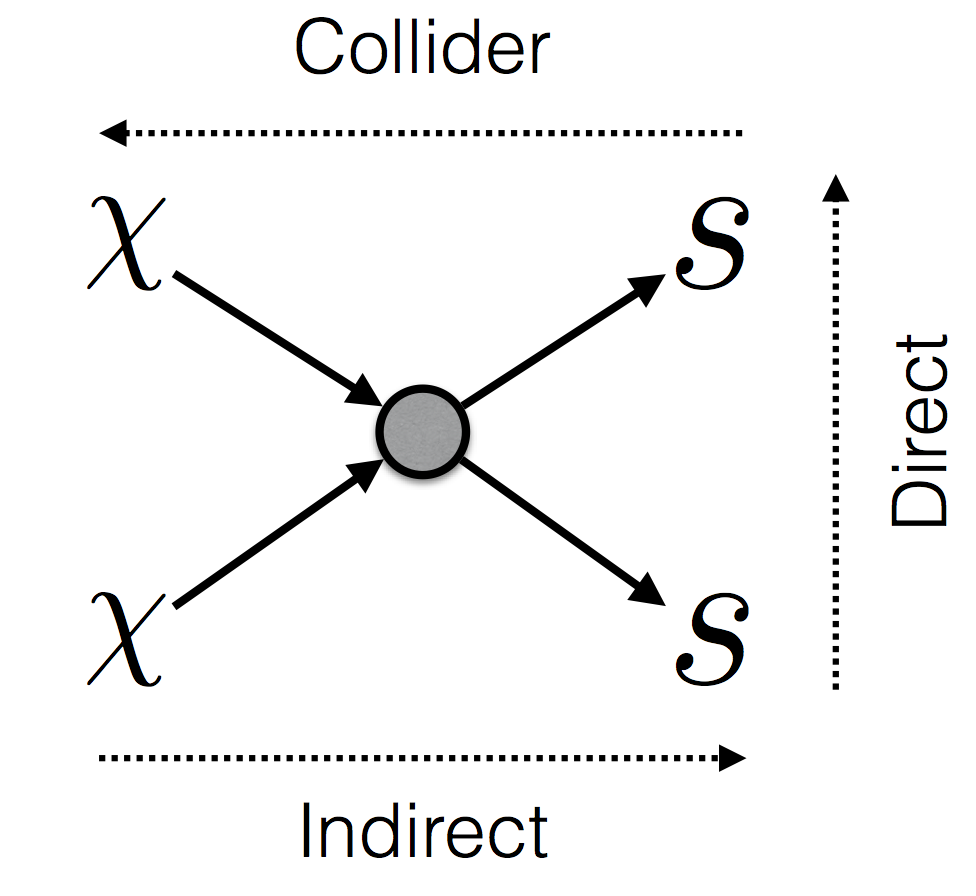
\includegraphics[width=0.45\textwidth]{images/3waystodetect/3waystodetect.pdf}
      \caption[Three Search Techniques]{
        The three general search techniques for dark matter.
        The $\chi$ is a dark matter particle, while $S$ is a standard model particle.
      }
      \label{fig:3_searches}
    \end{figure}
    
    In collider searches, $SS \rightarrow \chi\chi$, missing transverse energy is sought as dark matter particles are not expected to interact with the detector.
    For direct searches, $\chi S \rightarrow \chi S$, sensitive particle detectors are built deep underground.
    When a WIMP scatters off of a nucleus within the detector, the nuclear recoil can be observed, through signals such as crystal phonons, excitation and release of photons, or ionization.
    Being underground shields the detectors from cosmic rays, which create background collisions that can mimic WIMP signals.
    For example, in liquid xenon detectors, WIMP particle collisions in the liquid produce UV photons and electrons, which are used to infer the presence of the WIMPS~\cite{direct_lux,direct_xenon}.
    Another type are cryogenic, which use pucks of germanium and silicon to measure WIMP collisions.
    These collisions produce detectable ionization and phonon signals, which are used to classify the incident particle~\cite{direct_cdms}.
    A third example are scintillation detectors, which are built with crystals such as titanium-doped sodium iodine.
    When a WIMP collides with one of the nuclei within the crystal, that nucleus becomes excited, and then relaxes by releasing a photon~\cite{direct_dama}.
    However, to date no substantial dark matter signal has been detected with these methods~\cite{direct_dm_detection}.
    
    For indirect searches, $\chi\chi \rightarrow ss$, dark matter particles may annihilate or decay into standard model particles.
    Observatories then search for excesses of these particles, excesses that cannot be explained by currently understood astrophysics.
    This analysis searches for an excess of gamma rays, as the center of our galaxy is believed to host a dark matter halo.
    This spherical halo would allow for many $\chi\chi$ annihilations, producing gamma rays with
    
    $$\chi\bar{\chi} \rightarrow S\bar{S} \,,$$
    where $S\bar{S}$ can be any particle-antiparticle pair ($t\bar{t}$, $b\bar{b}$, $u\bar{u}$, $s\bar{s}$, \Pelectron{}\APelectron{}, \Pnue{}\APnue{}, \Pgg{}\Pgg{}, \Pg{}\Pg{}, \PHiggslight{}\PHiggslight{}, etc).
    The particle-antiparticle pairs then annihilate or decay into different spectra of photons ($\gamma$).
    These different annihilation channels can produce different spectra of gamma rays, which will also vary based on the WIMP mass and cross section chosen.
    This is described further in Section \ref{dm_spectral}.

\FloatBarrier

\section{Galactic Center}\label{sec:gc}
  
  The Galactic Center is a complex region of space, with many astrophysical sources of gamma rays.
  At its heart, kinematic observations of nearby stars have been used to infer the presence of a supermassive black hole, with a mass of \SI{4e6}{ M${{}_\odot}$ }~\cite{sgra_massdist}.
  Around this black hole, gamma ray emission is observed~\cite{gc_pointsrc_hess,gc_pointsource_hess2,gc_veritas_pointsource,gc_magic_pointsource}, though the production mechanism is still debated.
  There are other gamma-ray sources as well, including dust along the galactic plane and supernova remnants.
  The TeV gamma-ray emission from a few of these sources is visible in Figure~\ref{fig:hess_plane}.
  
  \begin{figure}[!t]
    \centering
    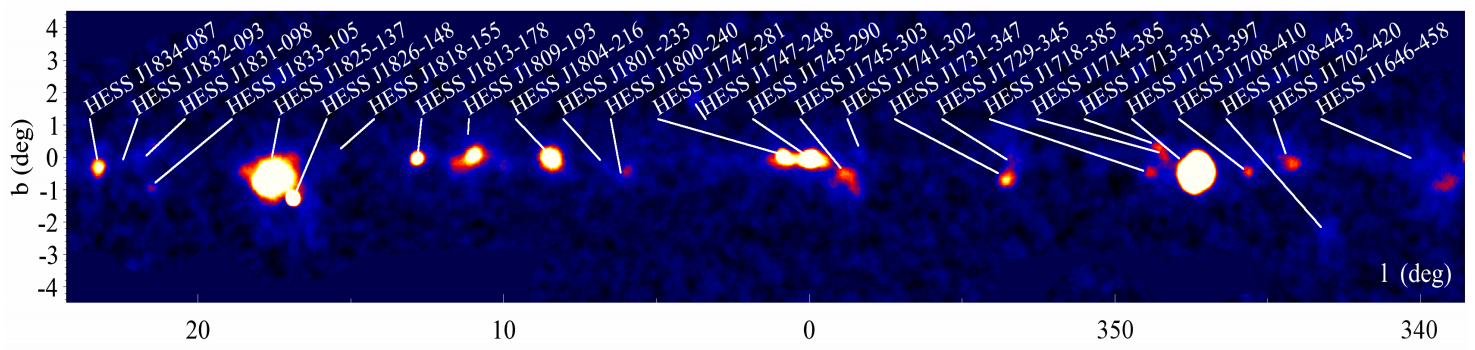
\includegraphics[width=0.98\textwidth]{images/hess_plane_survey/survey.pdf}
    \caption[HESS GC Survey]{
      Significance map of the Galactic Center, from the HESS Galactic Plane Survey~\cite{hess_gc_plane}.
      \CaptionBlankLine
    }
    \label{fig:hess_plane}
  \end{figure}
  
  \begin{figure}[!b]
    \centering
    \includegraphics[width=0.95\textwidth]{images/veritas_gc_ridge/ridge.pdf}
    \caption[VERITAS View of the Galactic Center Ridge]{
      Galactic Center Ridge, from Ref.~\cite{VeritasGCRidge2015}.
      \CaptionBlankLine
    }
    \label{fig:veritas_gc_ridge}
  \end{figure}

  The VERITAS significance sky map of this Galactic Center region is shown in Figure~\ref{fig:veritas_gc_ridge}.
  While a dark matter interpretation of this gamma-ray emission is intriguing~\cite{gc_pnt_is_dm1,gc_pnt_is_dm2}, there are several non-dark-matter models that might explain the observed features.
  One model that explains this TeV emission is that the supermassive black hole accelerates protons to PeV energies, which then collide with local atoms to produce \Ppizero{}s, which then decay into TeV gamma rays~\cite{gc_pevatron}.
  The second possibility suggests a nearby population of millisecond pulsars may be accelerating electrons, which then upscatter local photons to TeV energies~\cite{gc_pulsars,gc_pnt_is_not_dm2,gc_pnt_is_not_dm3}.
  The debate between these two models is currently ongoing~\cite{gc_pev_or_pwn}.
  Due to their limited angular resolution, the current generation of gamma-ray telescopes can only resolve the Galactic Center's gamma ray emission as a point source~\cite{VeritasGCRidge2015,gc_pointsrc_hess}.
  The Fermi telescope has observed a similar source of GeV gamma rays around the Galactic Center~\cite{gc_fermi_dm}, though neither the dark matter or millisecond pulsar explanations are completely conclusive~\cite{fermi_gc_pulsar_vs_dm,hoopergc}.
  
  In addition to this central source, there are also other sources of gamma rays in the vicinity.
  One of these sources is a disk of dust along the galactic plane, acting as an interaction medium for proton cosmic rays~\cite{diffusegamma1989}.
  These proton-proton collisions then produce neutral pions, which decay into gamma rays~\cite{hess_gc_diffuse}.
  High energy electrons scattering off of nuclei can also produce gamma rays via Bremsstrahlung.
  Gamma rays around the Galactic Center can also be produced by inverse Compton scattering.
  This occurs due to the upscattering of optical, infrared, and cosmic microwave background photons.
  These photons are upscattered by electrons accelerated in nearby sources such as pulsar wind nebulae.
  Supernova remnants can also produce gamma rays, as their expanding shells interact with ambient dust. 
  The extended emission from inverse Compton, pion decay, and supernovae processes are not modeled in this analysis.
  This is because the atmosphere's lack of uniformity overwhelms any diffuse emission in the residual sky maps\footnote{These residual maps are discussed in Section~\ref{subsec:likemax}.}.


\section{Indirect Dark Matter Search}
  For this analysis, it is necessary to understand how a terrestrial telescope can detect the presence of dark matter.
  Imaging atmospheric Cherenkov telescopes like H.E.S.S., MAGIC, and VERITAS can indirectly search for dark matter.
  These observatories attempt to detect gamma rays that are emitted when two dark matter particles annihilate.
  Because the rate of annihilation depends on the local dark matter density, the gamma-ray emission rate is affected by the radially-dependent structure of the dark matter halo.

  \subsection{Dark Matter and Gamma Rays}
    Primarily, indirect searches focus on annihilating WIMPs, as the predicted decaying WIMP produces a lower flux of standard model particles than annihilation.
    WIMPs may annihilate into any standard model particle-antiparticle pair, but most studies examine a WIMP annihilating into a quark-antiquark or gamma-ray photon pair~\cite{pdg2016}.
    These different annihilations produce different spectra of final gamma rays.
    The final spectrum of gamma rays used in this analysis is calculated in Section~\ref{dm_spectral}.
    After the gamma-ray spectrum is understood, the spatial distribution of the annihilations is also discussed in Section~\ref{dm_spatial}.
    The expected flux of gamma rays from a halo can then be calculated by combining these spatial and spectral models.
  
  \subsection{Spectrum of Gamma Rays from WIMP Annihilations}\label{dm_spectral}
    
    %   Fragmentation fractions of b quarks into weakly decaying 
    %   b-hadron species in Z->b\bar{b} decay, in p\bar{p} collisions at sqrt(s)=1.96 TeV
    %   http://pdg.lbl.gov/2018/reviews/rpp2018-rev-b-meson-prod-decay.pdf
    %   pg4: Table 85.1
    %   b Hadron  | Fraction at Z [%] | Fraction at p\bar{p}
    %   B+,B^0    |       41.2 ± 0.8  |  34.0 ± 2.1 
    %   B_s       |        8.8 ± 1.3  |  10.1 ± 1.5
    %   b baryons |        8.9 ± 1.2  |  21.8 ± 4.7
    
    % B^+ (ub_) Decay Modes http://pdg.lbl.gov/2018/listings/rpp2018-list-B-plus-minus.pdf
    %   -> \bar{D}^0 X : 79   ± 4
    %   -> D^- X       :  9.9 ± 1.2
    %   -> D^0 X       :  8.6 ± 0.7
    % B^- (u_b) Decay Modes (charge conjugates of B^+)
    %   -> D^0 X       : 79   ± 4
    %   -> D^+ X       :  9.9 ± 1.2
    %   -> \bar{D}^0 X :  8.6 ± 0.7
    % B^0 (d_b) Decay Modes http://pdg.lbl.gov/2018/listings/rpp2018-list-B-zero.pdf
    %   -> K^± anything : 78   ± 8
    %   -> \bar{D}^0 X  : 47.4 ± 2.8
    %   -> D^- X        : 36.9 ± 3.3
    %   -> D^0 X        :  8.1 ± 1.5
    
    % D^+ (cd_) Decay Modes http://pdg.lbl.gov/2018/tables/rpp2018-tab-mesons-charm.pdf
    %   -> \bar{K}^0 anything + K^0 anything : 61    ± 5
    %   -> K^- anything                      : 25.7  ± 1.4
    %   -> \mu^+ anything                    : 17.6  ± 3.2
    %   -> e^+ semileptonic                  : 16.07 ± 0.30
    %   -> \bar{K}^0 \mu^+ \nu_{\mu}         :  8.74 ± 0.19
    %   -> \bar{K}^0 e^+ \nu_e               :  8.73 ± 0.10
    % D^- (c_d) Decay Modes (charge conjuages of D^+)
    %   -> \bar{K}^0 anything + K^0 anything : 61    ± 5
    %   -> K^+ anything                      : 25.7  ± 1.4
    %   -> \mu^- anything                    : 17.6  ± 3.2
    %   -> e^- semileptonic                  : 16.07 ± 0.30
    %   -> \bar{K}^0 \mu^- \bar{\nu}_{\mu}   :  8.74 ± 0.19
    %   -> \bar{K}^0 e^-   \bar{\nu}_e       :  8.73 ± 0.10
    % D^0 (cu_) http://pdg.lbl.gov/2018/tables/rpp2018-tab-mesons-charm.pdf
    %   -> \bar{K}^0 anything + K^0 anything : 47   ± 4
    %   -> K^- anything                      : 45.7 ± 2.8
    %   -> K^- \pi^+ \pi^0                   : 14.2 ± 0.5
    %   -> K^- \pi^+ \pi^+ \pi^-             : 8.11 ± 0.15
    
    % K^+ (s_u) Decay Modes http://pdg.lbl.gov/2018/tables/rpp2018-tab-mesons-strange.pdf
    %   -> \mu^+ \nu_{\mu}       : 63.56 ± 0.11
    %   -> \pi^+ \pi^0           : 20.67 ± 0.08
    % K^- (su_) Decay Modes (charge conjugate of K^+)
    %   -> \mu^- \bar{\nu}_{\mu} : 63.56 ± 0.11
    %   -> \pi^- \pi^0           : 20.67 ± 0.08
    % K^0 (s_d) Decay Modes (http://pdg.lbl.gov/2018/listings/rpp2018-list-K-zero.pdf
    %   -> 
    % K^0_S Decay Modes 
    %   -> \pi^0 \pi^0 : 30.69 ± 0.05
    %   -> \pi^+ \pi^- : 69.20 ± 0.05 
    % K^0_L Decay modes
    %   -> \pi^± e^∓ \nu_e       : 40.55 ± 0.11
    %   -> \pi^± \mu^∓ \nu_{\mu} : 27.04 ± 0.07
    %   -> \pi^0 \pi^0 \pi^0     : 19.52 ± 0.12
    %   -> \pi^+ \pi^- \pi^0     : 12.54 ± 0.05
    
    % \pi^0 Decay Modes http://pdg.lbl.gov/2018/listings/rpp2018-list-pi-zero.pdf
    %   -> \gamma \gamma  : 98.823 ± 0.034
    
    % b->B mesons
    
    In order to calculate the gamma-ray brightness of the dark matter halo, the produced gamma-ray energy spectrum from WIMP annihilations must be known.
    Different annihilation channels can produce different spectra.
    For instance, the $\chi\chi \rightarrow \gamma\gamma$ channel will produce a spectrum with a single spike at the WIMP's mass, while the $\chi\chi \rightarrow \bbbar{}$ channel will produce a curved power law spectrum of photons, shown in Figure~\ref{fig:chichi_spectrum}.
    WIMP annihilations are expected to have multiple channels, where a population of WIMPs will annihilate into different channels with different probabilities.
    However, only the $\chi\chi \rightarrow \bbbar$ channel is considered for this analysis.
    
    Three example Feynman diagrams of WIMP annihilations that produce a \bbbar pair are shown in Figure~\ref{fig:neutralino_feynman}, adapted from Ref.~\cite{Jungman:1995df}.
    The particle $\tilde{f}$ is a supersymmetric fermion, the $Z$ is the Z boson, and $H$ is Higgs boson.
    The analysis in this thesis searches for a general \bbbar signal, rather than the specific signal from one of these Feynman diagrams.
    
    \begin{figure}[h]
      \centering
      \hfill
      \begin{minipage}{0.17\textwidth}\includegraphics[width=\linewidth]{images/feynman_neutralino/neutralino_superf.pdf}\end{minipage}\hfill
      \begin{minipage}{0.25\textwidth}\includegraphics[width=\linewidth]{images/feynman_neutralino/neutralino_zboson.pdf}\end{minipage}\hfill
      \begin{minipage}{0.25\textwidth}\includegraphics[width=\linewidth]{images/feynman_neutralino/neutralino_aghost.pdf}\end{minipage}\hfill
      \hfill
      \caption[WIMP Annihilation Feynman Diagrams]{
        Three example Feynman diagrams of neutralino annihilations that produce a \bbbar pair.
      }
      \label{fig:neutralino_feynman}
    \end{figure}

    After the desired channel is selected, the spectrum of photons produced by that channel is calculated.
    This is done by repeatedly simulating all the photons produced when the \bbbar quarks hadronize and decay into other particles.
    Several of these decay processes are shown in Table~\ref{tab:bpaths2}.
    In the table, the $\bar{b}$ hadronizes into \PBplus or \PBzero, which then decay into \PK and \PD mesons (plus some other particles $X$), and the \PD mesons also decay into \PK mesons.
    The \PK mesons can then decay into \Ppipm and \Ppizero mesons, and finally the \Ppizero{}'s decay into two photons.
    % for pion decays, see section 3.3 in arxiv:1508.05190 (and references therein)
    Though these pion decays are the dominant source of photons, these listed particles (as well as other unlisted ones) may produce additional photons through bremsstrahlung or annihilation mechanisms.
    All of the photons produced from pion decays, bremsstrahlung, and annihilations then make up a gamma-ray spectrum that is used in this analysis.
    
    \begin{table}
      \centering
      \begin{tabular}{ccll}
        Source                       & Branching                       & Products       & PDG \\
        (Quarks)                     & Ratio (\%)                      &                & Chapter \\ \hline
        $\bar{b}$                    & $\xrightarrow{ \mathrm{Hadronization} }$   & \PBp, \PBz     & \href{http://pdg.lbl.gov/2018/reviews/rpp2018-rev-b-meson-prod-decay.pdf}{$b$-Hadron Production}              \\ \hline
        \PBp     $(u\bar{b})$   & $\xrightarrow{ 79   \pm4   }$   & $\APDzero + X$ & \href{http://pdg.lbl.gov/2018/listings/rpp2018-list-B-plus-minus.pdf}{Charged B Mesons}          \\
        \PBz     $(d\bar{b})$ & $\xrightarrow{ 78   \pm8   }$   & $\PKpm + X$    & \href{http://pdg.lbl.gov/2018/listings/rpp2018-list-B-zero.pdf}{Neutral B Mesons}          \\
        \PBz     $(d\bar{b})$ & $\xrightarrow{ 47.4 \pm2.8 }$   & $\APDzero + X$ & \href{http://pdg.lbl.gov/2018/listings/rpp2018-list-B-zero.pdf}{Neutral B Mesons}          \\
        \PBz     $(d\bar{b})$ & $\xrightarrow{ 36.4 \pm3.3 }$   & $\PDminus + X$ & \href{http://pdg.lbl.gov/2018/listings/rpp2018-list-B-zero.pdf}{Neutral B Mesons}          \\ \hline
        \APDzero $(u\bar{c})$    & $\xrightarrow{ 45.7 \pm2.8 }$   & $\PKplus + X$  & \href{http://pdg.lbl.gov/2018/tables/rpp2018-tab-mesons-charm.pdf}{Charm Mesons}          \\
        \PDminus $(d\bar{c})$  & $\xrightarrow{ 25.7 \pm1.4 }$   & $\PKplus + X$  & \href{http://pdg.lbl.gov/2018/tables/rpp2018-tab-mesons-charm.pdf}{Charm Mesons}          \\ \hline
        \PKplus  $(u\bar{s})$  & $\xrightarrow{ 20.67\pm0.08}$   & $\Ppizero + \Ppiplus$  & \href{http://pdg.lbl.gov/2018/tables/rpp2018-tab-mesons-strange.pdf}{Strange Mesons} \\
        \PKminus $(\bar{u}s)$  & $\xrightarrow{ 20.67 \pm0.08 }$ & $\Ppizero + \Ppiminus$  & \href{http://pdg.lbl.gov/2018/tables/rpp2018-tab-mesons-strange.pdf}{Strange Mesons} \\ \hline
        \Ppizero $\left ( \frac{u\bar{u} - d\bar{d} }{\sqrt{2}} \right )$   & $\xrightarrow{ 98.823\pm0.034}$ & $\gamma + \gamma$ & \href{http://pdg.lbl.gov/2018/listings/rpp2018-list-pi-zero.pdf}{Neutral Pion} \\
        %$$ & $\xrightarrow{ \pm }$ & $$ \\
        %\APDzero    & $\xrightarrow{ 47  \pm4   }$ & $K^0 + \bar{K}^0 + anything $ \\
        %\PDminus    & $\xrightarrow{ 61  \pm5   }$ & $K^0 + \bar{K}^0 + anything$ \\
        % Numbers are from  the beginning of this subsection
      \end{tabular}
      \caption[$b$ Quark Production of Gamma Rays]{
        Table of decay modes and products, indicating several ways photons are produced from $\bar{b}$ quarks.
        The $X$ indicates other particles.
        Branching ratios and Particle Data Group (PDG) chapters are from Ref.~\cite{tanabashi2018review}.
      }
      \label{tab:bpaths2}
    \end{table}
    
    %\begin{table}
    %\centering
    %\begin{tabular}{lcll}
      %Source      & Branch Fraction                         & Products                  & Ref.     \\
      %\hline
      %$\bar{b}$   & $\xrightarrow{59.8   \% \pm 2.9    \%}$ & $\bar{D}^{0} + \textrm{other}$ &  \cite{pdg_2012} \\
      %$\bar{D}^0$ & $\xrightarrow{54.7   \% \pm 2.8    \%}$ & $K^+         + \textrm{other}$ &  \cite{pdg_2008} \\
      %$K^+$       & $\xrightarrow{63.56  \% \pm 0.11   \%}$ & $\mu^+ + \nu_{\mu}$            &  \cite{pdg_2014} \\
      %\hline
      %$\bar{b}$   & $\xrightarrow{23.3   \% \pm 1.7    \%}$ & $D^-   + \textrm{other}$       &  \cite{pdg_2012} \\
      %$D^-$       & $\xrightarrow{25.7   \% \pm 1.4    \%}$ & $K^+   + \textrm{other}$       &  \cite{pdg_2008} \\
      %$K^+$       & $\xrightarrow{63.56  \% \pm 0.11   \%}$ & $\mu^+ + \nu_{\mu}$            &  \cite{pdg_2014} \\

      %$K^+$     & $\xrightarrow{20.67  \% \pm 0.08   \%}$ & $\pi^0 + \pi^+$                &  \\
      %$\pi^0$   & $\xrightarrow{98.798 \% \pm 0.032  \%}$ & $\gamma + \gamma$              &  \\
      %$\pi^+$   & $\xrightarrow{99.9877\% \pm 0.00004\%}$ & $\mu^+ + \nu_{\mu}$            &  \\
      %Hadronization & $\bar{b}$ & $\xrightarrow{40.1   \% \pm 0.8    \%}$ & $B^+$                     &  \cite{pdg_2012} \\
      %Decay         & $B^+$     & $\xrightarrow{10.99  \% \pm 0.28   \%}$ & $l^+ + \nu_l + \other$    &  \cite{pdg_2014} \\
      %\hline
      %Hadronization & $\bar{b}$ & $\xrightarrow{40.1   \% \pm 0.8    \%}$ & $B^0$                     &  \cite{pdg_2012} \\
      %Decay         & $B^0$     & $\xrightarrow{10.33  \% \pm 0.28   \%}$ & $l^+ + \nu_l$             &  \cite{pdg_2014} \\
      %\hline
      %Hadronization & $\bar{b}$ & $\xrightarrow{ 9.3 \% \pm 1.6 \%}$ & $\bar{b}\bar{q}\bar{q}$   \\
      %Hadronization & $\bar{b}$ & $\xrightarrow{10.5 \% \pm 0.6 \%}$ & $B^0_S$                \\
      %$\bar{b}$ & $\xrightarrow{17.3 \% \pm 2.0 \%}$ & $D^{*}(2010)^{+} + \any$ & \\
      %$D^0$     & $\xrightarrow{6.53 \% \pm 0.17\%}$ & $e^{+}           + \any$ & \\
      %$D^0$     & $\xrightarrow{6.7  \% \pm 0.6 \%}$ & $\mu^{+}         + \any$ & 
      %Decay & $D^0$     & $\xrightarrow{47   \% \pm 4   \%}$ & $\bar{K}^0 + K^0 + \any$     & inclusive \\
      %Decay & $D^-$     & $\xrightarrow{61   \% \pm 5   \%}$ & $\bar{K}^0 + K^0 + \any$     & inclusive \\
    %\end{tabular}
    %\caption[$b$ Quark Production of Photons]{
      %Table of decay modes and products, indicating two ways ways a lone $b$ quark can indirectly produce photons.
      %The $\mu^+$ is then able to produce bremsstrahlung photons.
      %The charge conjugate of the source is assumed to charge conjugate the products.
      %Constituent quarks for particles are $\bar{D}^0=\bar{c}u$, $K^+=u\bar{s}$, and $D^-=\bar{c}s$.
      %$B^+=u\bar{b}$, $B^0=d\bar{b}$, $B^0_S=s\bar{b}$, $D^0=c\bar{u}$, $K^-=\bar{u}s$, $\pi^0=\frac{u\bar{u}-d\bar{d}}{\sqrt{2}}$, and $\pi^+=u\bar{d}$.
      %}
    %\label{tab:bpaths}
    %\end{table}
    
    The software package CLUMPY~\cite{CLUMPYcode} is used in this thesis to calculate the gamma-ray spectra for each annihilation channel.
    The spectral models that CLUMPY uses are based on the annihilation spectra in the PPPC 4 DM ID~\cite{pppc4_dm_spectra,pppc4_ewcorrections}.
    These spectra are calculated using Monte Carlo simulations performed with PYTHIA~\cite{pythia} and HERWIG~\cite{herwig}.
    Figure~\ref{fig:chichi_spectrum} shows the resultant spectra from the annihilation of two WIMPs.
    Each line shows the spectrum from a different initial WIMP mass.

    \begin{figure}[bt]
      \centering
      \includegraphics[width=0.95\textwidth]{images/spectra/chichi_spectrum.pdf}
      \caption[Single Annihilation Spectra]{
        Resultant photon spectra from the annihilation of two WIMP particles solely into the \bbbar channel.
        Each colored line represents a different WIMP mass.
      }
      \label{fig:chichi_spectrum}
    \end{figure}

    These spectra can be combined with the J factor (Equation~\ref{eqn:jfactor}) to calculate the gamma-ray flux produced by the halo (Equation~\ref{eqn:dmflux}).
    It is important to note that mass-to-light ratios, and their derived J factors are usually inferred from measuring star spectra.
    These measured J factors can therefore suffer from large errors, as it can be difficult to determine which stars are within a target gravitational well, and which ones are foreground or background stars~\cite{segue_jfactor_errors}.
    
    By using estimated parameters with Equation~\ref{eqn:dmflux}, the flux of gamma rays from a dark matter halo can be estimated in order to understand how few events a dark matter halo produces.
    The flux of gamma rays from a dark matter halo can be estimated with Equation~\ref{eqn:dmflux} to understand how just how few gamma rays can be observed from a dark matter halo.
    For this estimate, the dark matter mass is chosen to be \SI{10}{\TeV{}}, and the velocity-averaged cross section $\left < \sigma v \right >$ is set at the relic cross section.
    Other chosen parameters are specified in Table~\ref{tab:halo_nphotons}, to align with the VERITAS telescope performance, or the parameters of the dark matter analysis performed in later chapters.
    For the table parameters, the dark matter halo would only produce a VERITAS-detectable gamma ray between \SIrange{4}{70}{\TeV{}} every 39 hours.
    This flux $\Phi$ is proportional to the $\sv$, so a factor of $n$ larger particle cross section would produce a factor of $n$ larger photon flux.
    Another way to increase the observed photon flux is by expanding the observable gamma-ray energy range.
    If the entire VERITAS energy range of \SIrange{1.5}{70}{\TeV{}} is used, the integrated photon spectrum between \SIrange{1.5}{10}{\TeV{}} increases, and the observed halo photon flux also increases by a factor of 26.
    
    \begin{table}[]
      \centering
      \begin{tabular}{r|l}
        \hline
        \textbf{Estimated Parameters}            & \\
        $m_{\chi}$                               & \SI{10}{\TeV{}}         \\
        Relic velocity-averaged cross section $\vacs$ & \SI{3e-26}{cm^3/s}   \\
        Field of view                            & \ang{3}              \\
        Detectable photon energy range           & \SIrange{4}{70}{\TeV{}} \\
        Observatory effective area               & \SI{287000}{m^2}     \\
        Annihilation channel                     & $\chi\chi \rightarrow \bbbar $ \\
        Dark matter halo shape                   & Einasto              \\
        \hline
        \textbf{Derived Values}                  & \\
        Integrated photon spectrum : $\int \frac{dN_{\gamma}}{dE} dE$        & 0.00536 photons per $\chi\chi$ annihilation \\
        J factor :$\int \int \rho^2 dl\,d\Omega$ & \SI{3.88e22}{\GeV{}^2/cm^5}      \\
        Halo flux $\Phi$                         & \SI{2.5e-11}{photons/(s*m^2)} \\
        One halo photon detected every           & \SI{39}{hours} \\
        \hline
      \end{tabular}
      \caption[Halo Model Parameters]{
        Number of gamma rays from a dark matter halo.
        Field of view is the radial field of view of VERITAS.
        Observatory effective area is the VERITAS effective area at \ang{29} telescope elevation (the average elevation of Galactic Center at VERITAS's latitude), \ang{0.5} offset from GC, at the $\log_{10}$ mean energy (\SI{16.7}{\TeV{}}) in the selected energy range.
        The Einasto halo shape parameters are chosen to be the same as in Section~\ref{dm_spatial}.
      }
      \label{tab:halo_nphotons}
      % values derived with $VERIPY/thesis/analysis/example_dm_halo_photons/example.py
    
    \end{table}

    \FloatBarrier

  \subsection{Dark Matter Halo Structure}\label{dm_spatial}
    
    Observations allow most galactic dark matter halos to be modeled using a class of similar density profiles.
    A currently favored profile is the Einasto profile~\cite{einastoprofile1,einastoprofile2}.
    This profile describes the mass-density of dark matter at a distance $r$ from the halo center, $\rho(r)$.
    The Einasto profile is described by

    \begin{equation} \label{eqn:einasto}
      \rho_{\textrm{DM}} \left( r \right) = \rho_{s} Exp \left( - \frac{2}{\alpha} \left( {\left( \frac{r}{r_s} \right)}^{\alpha} - 1 \right) \right) \,,
    \end{equation}
    where $r_s$ is the scale radius of the halo, which specifies how wide the dark matter halo is.
    The parameter $\rho_s$ is the scale density, which is the dark matter density at the scale radius.
    The parameter $\alpha$ is the power of the density profile's slope.
    
    A larger $\alpha$ reduces the dark matter densities above and below the scale radius $r_s$.
    Both $\alpha$ and $r_s$ are from the best fit values of the Aq-A-1 simulation in Table 2 of Ref.~\cite{mw_halo_params}.
    The $r_s$ parameter is calculated via $r_s=r_{-2}=15.14\:\textrm{kpc}$, where $r_{-2}=\frac{11.05}{h_{73}}\:\textrm{kpc}$ (in Ref.~\cite{mw_halo_params}, Table 2) and $h_{73}=0.73$ from Section 2.1 in Ref.~\cite{mw_halo_params}.
    In the model, the parameter $\alpha$ is fixed to 0.17, and $r_s$ is fixed to \SI{15.14}{kpc}.
    The distance to the Galactic Center is known to be $r_\odot=8\:\textrm{kpc}$~\cite{gc_distance_1,gc_distance_2,gc_distance_3}.
    The assumed Milky Way mass profile has a mass density of $\rho_\odot = 0.4\:\frac{\textrm{GeV}}{\textrm{cm}^3}$~\cite{local_dm_density,direct_dm_astrophysical_uncertainties}.
    Since $r_\odot$ and $\rho_\odot$ are known, then in Equation~\ref{eqn:einasto} the dark matter density at the scale radius $\rho_s$ is derived to be \SI{0.12}{\GeV{}\per\cm^3}.
    With these values, the Einasto profile in Equation~\ref{eqn:einasto} is shown in Figure~\ref{fig:gchalo_density}.
    The distribution of dark matter follows an Einasto profile.
  
    \begin{figure}[!t]
      \centering
      \includegraphics[width=0.85\textwidth]{images/halo/gc_einasto_profile.pdf}
      \caption[Galactic Center Einasto Halo Density]{
        Mass density of the Einasto dark matter halo (Equation~\ref{eqn:einasto}) used in this analysis.
        The bottom x axis shows the angle (as viewed from Earth) from the Galactic Center, while the top x axis shows the distance from the Galactic Center in kiloparsecs.
        \CaptionBlankLine
        }
      \label{fig:gchalo_density}
    \end{figure}

    
    Most n-body simulations predict that density profiles steeply rise as $r \rightarrow 0$, forming a peak or \textit{cusp} at their center.
    However, observations of dwarf galaxies usually show a flat density core within a given radius~\cite{flores1994observational,CoreVsCusp}.
    This may be due to the presence of baryons in this core region, which can diffuse the central cusp of WIMPs into a core-like shape~\cite{corecusp_baryondiffuse1,corecusp_baryondiffuse2}.
    As this flat core occurs in the innermost region covered by the gamma-ray observations in this analysis, the choice of a cusped or cored dark matter halo can have a significant impact.
    Specifically, if the true dark matter halo has a cored profile, but is modeled using a cusped one, then any derived upper limits on the dark matter cross section would be different.
    As a basic first step, only a cusped halo is used in this thesis.
    
    When choosing which dark matter target to observe with a gamma-ray observatory, knowing the gamma-ray brightness of different sources can be useful.
    This Einasto density profile can be integrated to calculate the gamma-ray brightness, independent of the WIMP model being searched for.
    For annihilating dark matter, $\rho_{\textrm{DM}}\left(r\right)^2$ must be integrated along the line of sight.
    
    The flux of gamma rays produced by these annihilations is given by
    
    \begin{equation}\label{eqn:dmflux}
      \frac{ d\Phi }{ dE d \Omega } = \frac{ \left \langle \sigma v \right \rangle }{8 \pi m_\chi^2} \frac{dN_{\gamma}}{dE} \int \rho^2 dl \, ,
    \end{equation}
    where the photon flux $\Phi$ is the number of gamma rays detected per $\textrm{area}\times\textrm{time}$.
    The velocity-averaged cross section of the dark matter candidate is $\left \langle \sigma v \right \rangle$.
    Velocity-averaging is used because the cross section is velocity dependent, and the WIMPs that pass through a volume of space will have a distribution of velocities~\cite{wimp_veldist}.
    The average spectrum of photons produced by a single $\chi\chi$ annihilation is $\frac{dN_{\gamma}}{dE}$.
    The density integral in Equation~\ref{eqn:dmflux} with the solid angle $d\Omega$ differential is often calculated separately, and is referred to as the $J$ factor,

    \begin{equation}\label{eqn:jfactor}
      J = \int \rho^2 dl\,d\Omega \;\; .
    \end{equation}

    The $J$ factor is used to compare the relative gamma-ray brightness of different dark matter halos, which is a function of both dark matter density and observing distance.
    The Einasto density in Equation~\ref{eqn:einasto} can be integrated to calculate the $J$ factor at various radii, which is shown in Figure~\ref{fig:gchalo_jfactor}.
    In Figure~\ref{fig:gchalo_jfactor}, the profile shown is calculated with Equation~\ref{eqn:jfactor}, where the $d\Omega$ integration limits span an angle of \ang{0.01}.
    This J-factor profile then forms the spatial component of the dark matter halo, $M_{s,\textrm{halo}}$, used in Chapter~\ref{chapter:analysis}.
    This profile is shown in a two-dimensional plot in Figure~\ref{fig:halojfactor}.
    
    \begin{figure}[!t]
    \centering
      \includegraphics[width=0.85\textwidth]{images/halo/gc_einasto_jfactor.pdf}
      \caption[Galactic Center Einasto Halo J-Factor]{
        J-factor profile as a function of angle from the Galactic Center, calculated via Equation~\ref{eqn:jfactor} with the Einasto density profile in Equation~\ref{eqn:einasto}.
        The J-factor values are calculated by integrating \ang{0.01} around each angle from the Galactic Center.
      }
      \label{fig:gchalo_jfactor}
    \end{figure}
  
  \begin{figure}[!t]
    \centering
    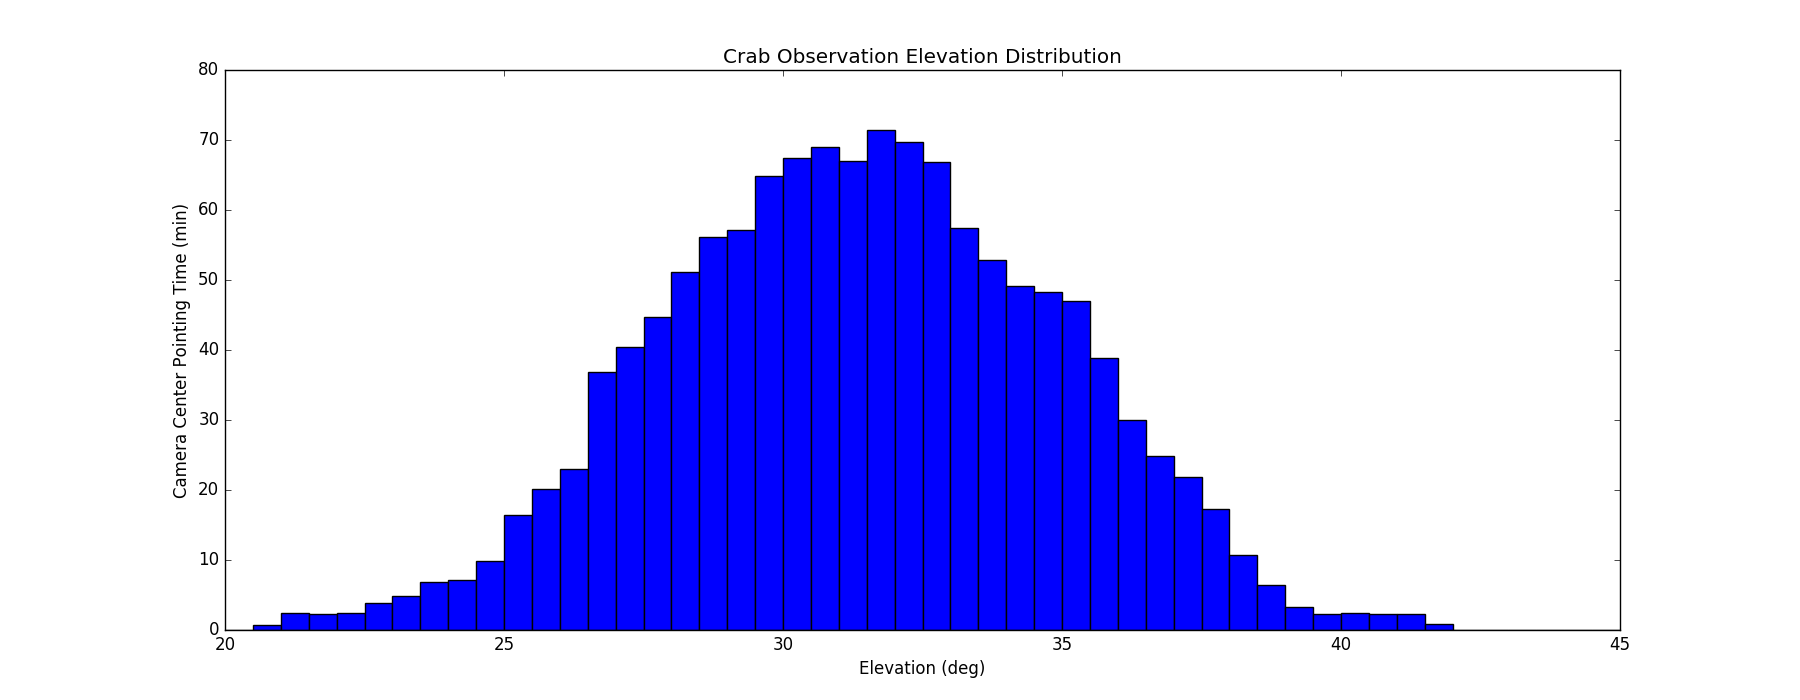
\includegraphics[width=0.85\textwidth]{images/halo_flux/plot.pdf}
    \caption[Galactic Center Halo J-Factor Sky Map]{
      J-factor of the dark matter halo model used in this analysis.
      The green circles indicate the different observation regions.
      Note this is showing the same model as Figure~\ref{fig:gchalo_jfactor}, except here the J-factor axis is linear instead of logarithmic.
      The black corners result from the halo model only being calculated out to a radius of \ang{3}, since there are no observations that extend past that.
    }
    \label{fig:halojfactor}
  \end{figure}

  The halo structure in Figure~\ref{fig:halojfactor} is a simple first step halo, one that does not account for more complex dark matter models.
  For example, a search for decaying dark matter would instead change the J-factor calculation to $\int \rho \, dl$, spreading out the gamma-ray emission.
  More exotic WIMP models may slightly alter the gamma-ray brightness of the dark matter halo, compared to the previously mentioned WIMP model.
  For example, if dark matter WIMPs have an attractive force between them, their effective annihilation cross section is enhanced, increasing the gamma-ray emission from the halo.
  This effect is called Sommerfeld enhancement~\cite{sommerfeld}.
  % originally from http://inspirehep.net/record/1286230/files/Thesis-2009-Nierop.pdf
  % from http://www.pnas.org/content/112/40/12264.full.pdf
    
  
  \FloatBarrier
    
\section{Cherenkov Photons}\label{sec:cherenkov}

  Cherenkov light and its production is discussed in this section, because the detection of gamma rays in Section~\ref{sec:atmoshowers} relies heavily on knowledge of Cherenkov light.
  Within the Earth's atmosphere (or any dielectric medium), the phase velocity of light $c_{atmosphere}$ is slightly slower than in a vacuum.
  Any charged particles travelling at velocity $v > c_{atmosphere}$ will induce the atmosphere to produce Cherenkov photons~\cite{cherenkov}.
  From a single charged particle of constant velocity, Cherenkov photons form a conical wavefront shown in Figure~\ref{fig:cherenkovangle}.
  This wavefront is similar to a sonic boom shockwave, or the wake produced when a boat travels faster than the speed of the waves.

  \begin{figure}[!t]
    \centering
    \includegraphics[width=0.27\textwidth]{images/cherenkov_angle/cherenkovangle.pdf}
    \caption[Cherenkov Emission Angle]{
      Cherenkov light (blue arrows) is emitted at angle $\theta$, relative to the charged particle z's path.
    }
    \label{fig:cherenkovangle}
  \end{figure}

  Cherenkov photons are emitted at an angle $\theta$ relative to the charged particle's path, determined by the index of refraction of the medium $n$, the speed of the charged particle $v$, and the speed of light in the medium $c$:
  % showers are 10km up, light pool on ground is 130m diameter, \theta = ArcSin(130/10000) * 180 / pi = 0.73deg ~ 1deg

  \begin{equation}\label{eqn:cherenkovangle}
    \theta = ArcCos \left ( \frac{c}{n \; v} \right ) \,.
  \end{equation}
  
  For the air showers used in this analysis, the Cherenkov angle $\theta$ is \nicetilde\ang{1}.
  In practice, air showers are more complex due to the number and distribution of charged particles and their velocities, as well as energy losses.
  These effects tend to smear the theoretically-clean Cherenkov cones into a diffuse pool of light on the ground, shown in Figure~\ref{fig:lightpool}.

  \begin{figure}[!t]
    \centering
    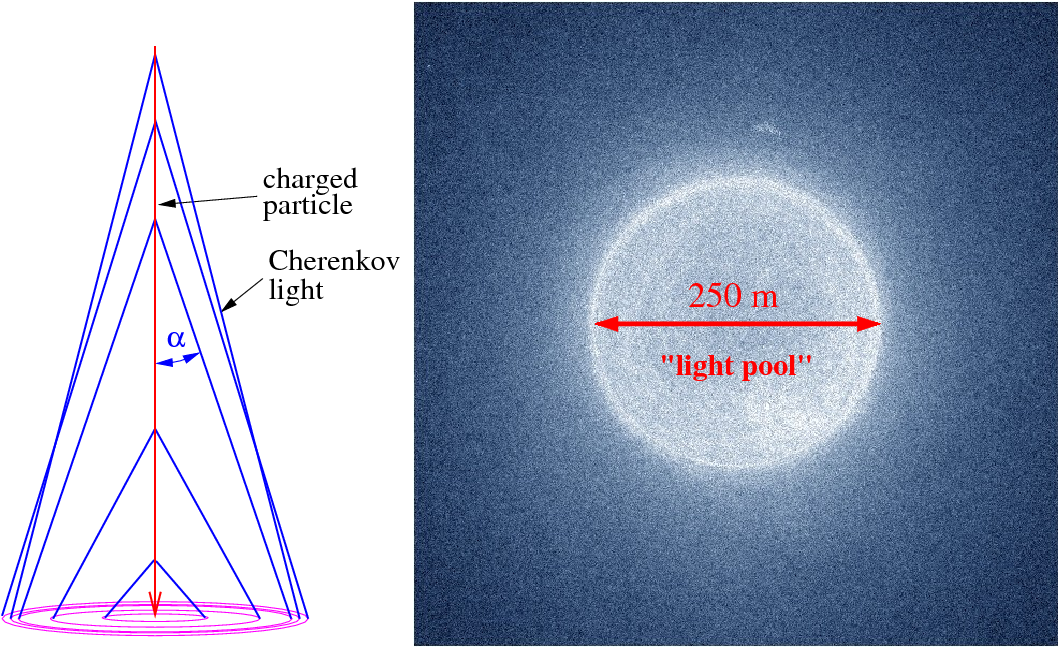
\includegraphics[width=0.85\textwidth]{images/lightpool/lightpool.pdf}
    \caption[Cherenkov Light Pool]{
      Cherenkov light from a gamma ray shower illuminating the ground.
      Due to the changing atmospheric density, the Cherenkov angle changes as the electromagnetic shower descends (left), concentrating the emitted light into a ring-like pool (right).
      The initial gamma ray in this simulated example had an energy of \SI{1}{\TeV{}}.
      Figure is from Ref.~\cite{Voelk}.
    }
    \label{fig:lightpool}
  \end{figure}
  
  The spectrum of photons produced by the Cherenkov effect can be calculated with the Frank-Tamm formula~\cite{franktamm1,franktamm2},
  
  \begin{equation}\label{eqn:franktamm}
    \frac{dE}{dx\,d\omega}=\frac{(ze)^2 \, \omega}{c^2} \left ( 1 - \frac{c^2}{v^2 \;\epsilon(\omega)} \right ) \,,
  \end{equation}
  where $E$ is the energy emitted as Cherenkov radiation, $x$ is the length of the charged particle path, $ze$ is the charge of the particle, $\omega$ is the emitted Cherenkov photon frequency, $c$ is the speed of light (phase velocity) in the medium, $v$ is the speed of the particle, and $\epsilon(\omega)$ is the frequency-dependent permittivity.
  
  \begin{figure}[!t]
    \centering
    \includegraphics[width=0.65\textwidth]{images/CherenkovReactor/cherenkovreactor.eps}
    \caption[Cherenkov Light from a Reactor]{
      Blue Cherenkov light in the Advanced Test Reactor core, at the Idaho National Laboratory~\cite{cherenkovreactor,atrlab}.
    }
    \label{fig:cherenkovreactor}
  \end{figure}
  
  In Figure~\ref{fig:cherenkovreactor}, a visible example of Cherenkov photons is shown, produced in the Advanced Test Reactor at the Idaho National Laboratory.
  Neutrons emitted by the reactor collide with atoms in the water, freeing some electrons with enough kinetic energy to travel faster than the speed of light in water.
  These superluminal-in-water electrons then create the blue Cherenkov photons imaged here.
  
  Section~\ref{sec:atmoshowers} covers how particles from outer space can produce Cherenkov photons.
  These UV- and visible-spectrum Cherenkov photons are then imaged and recorded by the VERITAS observatory, as discussed in Chapter~\ref{chapter:veritas}.
  
    
\section{Atmospheric Showers}\label{sec:atmoshowers}

  When a particle (the primary) strikes an atom of Earth's atmosphere at GeV or higher energies, it sets off a cascade of energetic particles called an air shower~\cite{Bethe1934,Klein1999}.
  When the primary particle consists of one or more hadrons, like a proton or iron atom, it creates a hadronic shower.
  When the primary particle is a gamma ray or a charged lepton, it creates an electromagnetic shower.
  Electromagnetic showers produce a cascade of electrons, positrons ($e^{+}$), and photons, where each successive generation of particles tends to have more particles but less energy per particle than the last.
  To start the shower, the primary gamma ray will interact with an atmospheric atom, producing an $e^{-}e^{+}$ pair, each with roughly half the primary gamma ray's energy, as shown in Figure~\ref{fig:emcascade}.
  The $e^{-}$ and $e^{+}$ emit bremsstrahlung photons, and incite the atmosphere to emit Cherenkov photons, discussed further in Section~\ref{sec:cherenkov}.
  The higher-energy bremsstrahlung photons then produce $e^{-}e^{+}$ pairs, which go on to produce more bremsstrahlung and Cherenkov photons.
  As each newly created particle has less energy than its parent particle, eventually the particles in the shower lack the energy to produce additional child-particles.
  When electrons have around \SI{80}{\MeV{}}\footnote{This is the energy for which, for an electron, the loss of energy due to ionization is equal to the loss of energy due to bremsstrahlung~\cite{tanabashi2018review,berger196410}} or less of kinetic energy, energy losses due to ionization begin to dominate~\cite{pdg_2014}.

  \begin{figure}[t]
    \centering
    \includegraphics[width=0.95\textwidth]{images/cascade_diagram/feynman/cascade.pdf}
    \caption[Electromagnetic Cascade]{
      Diagram of the first few generations of an electromagnetic cascade as it descends downwards through the atmosphere, layered by interaction generation~\cite{ellis2017tikz}.
      At the top of the diagram, $\gamma{}_o$ is the initial astrophysical gamma ray.
      \CaptionBlankLine
    }
    \label{fig:emcascade}
  \end{figure}

  Of all detected air showers, \nicetilde{}99\% are due to protons and electrons, rather than gamma rays.
  Protons produce hadronic showers which also produce Cherenkov light, like electromagnetic showers.
  In the initial collision, the astrophysical proton $p_{\textrm{cosmic}}$ interacts with an atmospheric nucleon $N$.
  The proton-nucleon collision then may produce pions ($\pi^{\pm}$ and $\pi^{0}$), as well as other particles whose production rates vary with available interaction energy.
  These other particles include additional protons and neutrons, as well as kaons, other mesons, and additional baryons and nucleons.
  These all go on to interact and decay to produce further particles, as part of a hadronic cascade.

  %\begin{equation}\label{eqn:protoncollision}
    %p_{\textrm{cosmic}} + p_{\textrm{atmo}} \rightarrow \pi^+ + \pi^+ + \pi^0 + X \;\;,
  %\end{equation}
  
  The $\pi^0$ decays into two gamma rays, which produce an electromagnetic cascade of electrons, positrons, and lower-energy photons.
  After each generation of the hadronic cascade, roughly 1/3 of the shower's energy is transferred into a new electromagnetic sub-shower.
  %The interaction produces $\pi^+\pi^+\pi^0$, where each particle receives \nicetilde $\frac{1}{3}$ of the initial proton's energy.
  This $\pi^{0}$ decay is shown in Figure~\ref{fig:feynman_pi}.
  
  \begin{figure}[tb]
    \centering
    \hfill
    \begin{minipage}{0.45\textwidth}\includegraphics[width=\linewidth]{images/feynman_particles/pion_gamma.pdf}\end{minipage}\hfill
    \begin{minipage}{0.45\textwidth}\includegraphics[width=\linewidth]{images/feynman_particles/pionplus.pdf}  \end{minipage}\hfill
    \hfill\hfill
    \caption[Feynman Diagrams of Pions]{
      Left: Feynman diagram of a $\pi^{0}$ decaying into two photons.
      Right: Feynman diagram of $\pi^{+}$ decaying into a lepton pair.
      \CaptionBlankLine
    }
    \label{fig:feynman_pi}
  \end{figure}
      

  %\begin{figure}[!ht]
  %  \centering
  %  \includegraphics[width=0.5\textwidth]{images/feynman_particles/pion_gamma.pdf}
  %  \caption[Feynman Diagram of $\pi^{0}$ Decay]{
  %    Feynman diagram of a $\pi^{0}$ decaying into two photons.
  %    \CaptionBlankLine
  %  }
  %  \label{fig:feynman_pi0}
  %\end{figure}

  %\begin{figure}[!hb]
  %  \centering
  %  \includegraphics[width=0.5\textwidth]{images/feynman_particles/pionplus.pdf}
  %  \caption[Feynman Diagram of $\pi^{+}$ Decay]{
  %    Feynman diagram of $\pi^{+}$ decaying into a lepton pair.
  %    %\CaptionBlankLine
  %  }
  %  \label{fig:feynman_piplus}
  %\end{figure}
  
  % see here for neutron: https://en.wikipedia.org/wiki/Cosmic_ray
  In hadronic showers, any produced \pip{}s and \pim{}s can travel far in the transverse direction, away from the main axis of the primary particle.
  The \pip{}s and \pim{}s then decay into $\mu^{+}\nu_{\mu}$ and $\mu^{-}\bar{\nu}_{\mu}$ pairs, respectively.
  The \pip{} decay is shown in Figure~\ref{fig:feynman_pi}.
  The \pio{} quickly decays into a pair of gamma rays, each of which then start their own electromagnetic shower.
  The \pip{} and \pim{} have longer lifetimes ($\pi^{\pm} \rightarrow $\SI{3e-8}{s} vs $\pi^{0} \rightarrow $\SI{9e-17}{s}~\cite{pdg_2014}), allowing them to carry energy farther away from the central shower axis.
  Both of these effects create sub-showers farther away from the primary particle axis, which tends to cause hadronic showers, and their resulting Cherenkov images, to be wider than a purely electromagnetic shower of the same length. 

  In order to accurately measure the gamma rays from an astrophysical source, the hadronic showers must first be removed.
  Because hadronic showers produce a slightly different image of Cherenkov light, many of them can be excluded from the analysis.
  The process of identifying and excluding these hadronic showers is referred to as gamma-hadron separation.
  
  In Figure~\ref{fig:gamma_vs_proton_airshower}, the differences between a gamma-ray shower (left) and a proton shower (right) are shown.
  Darker areas indicate more Cherenkov photons are produced by charged particles in the shower.
  The gamma-ray shower produces most of its Cherenkov photons along the central vertical core of the shower, while the proton shower produces Cherenkov photons spread out in a wider, fan-like shape.
  In the proton shower, any produced \pio{}'s decay into electromagnetic sub-showers in the interior of the shower.
  The net effect is that, when compared to a gamma ray, a proton must start with \nicetilde{}3 times the energy to produce a similar amount of Cherenkov photons, which are distributed in a wider pattern.

  \begin{figure}[!b]
    \centering
    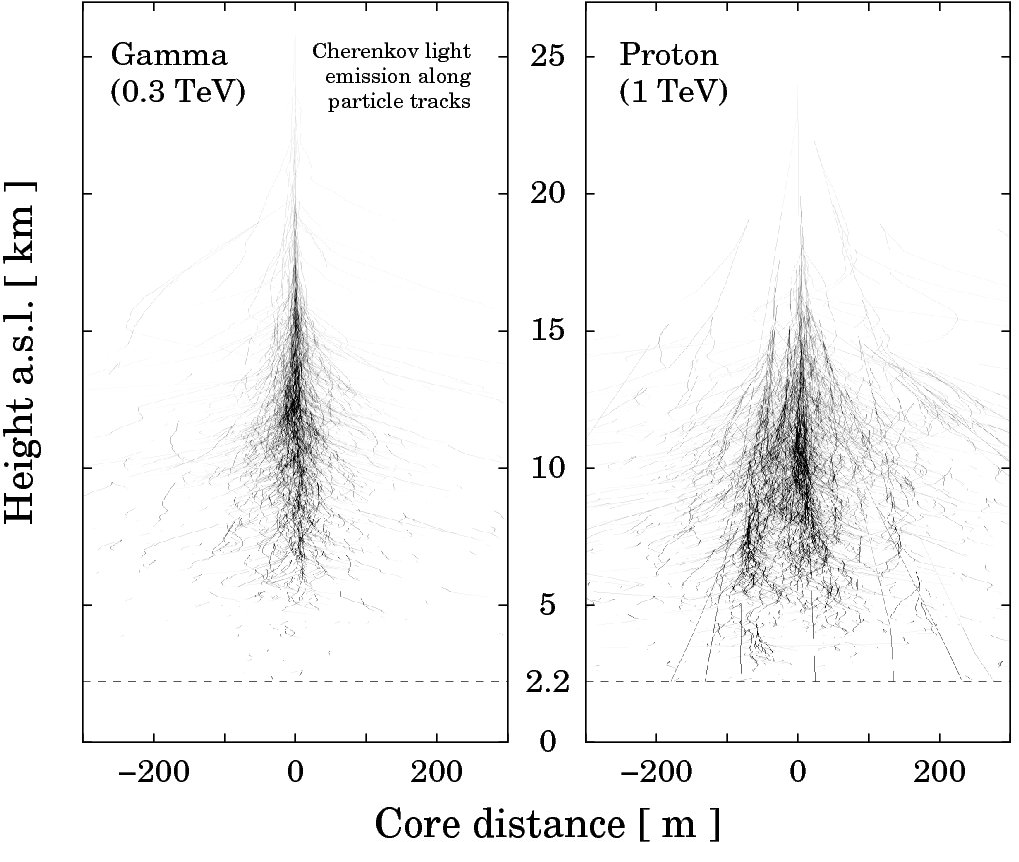
\includegraphics[width=0.7\textwidth]{images/showers_gamma_proton}
    \caption[Gamma Ray and Proton Showers]{
      A gamma ray shower (left) alongside a proton shower (right)~\cite{Bernlohr2008149}.
    }
    \label{fig:gamma_vs_proton_airshower}
  \end{figure}
  
  \FloatBarrier

